% Exemplo de relatório tecnico do IC (http://www.ic.unicamp.br/~reltech)

\documentclass[12pt,twoside]{article}
\usepackage{techrep-ic}

\usepackage[brazil]{babel}
\usepackage[utf8]{inputenc}

\usepackage{indentfirst}
\usepackage{tikz}
\usepackage{caption}
\usepackage{subcaption}

\usepackage
[pdftitle={Avaliacao do Impacto de Tecnicas de Formacao de Regioes no Gerenciamento de Code cache},
pdfauthor={G. Vieira, A. Carvalho, G. Piccoli, G. Valente, J. de Lucca},
pdfsubject={Relatorio Final},
pdfkeywords={VMs, Region Formation, Code Cache, RAIn, x86},
pdfpagemode={UseNone},
bookmarks,
pdfstartview={FitH},
colorlinks,
linkcolor={black},
citecolor={black},
urlcolor={blue},
hyperindex]
{hyperref}



\usepackage{listings}

\lstset{
  backgroundcolor=\color{white},   % choose the background color; you must add \usepackage{color} or \usepackage{xcolor}
  basicstyle=\footnotesize\ttfamily,        % the size of the fonts that are used for the code
  breakatwhitespace=false,         % sets if automatic breaks should only happen at whitespace
  breaklines=true,                 % sets automatic line breaking
  captionpos=b,                    % sets the caption-position to bottom
  commentstyle=\color{mygreen},    % comment style
%  deletekeywords={...},            % if you want to delete keywords from the given language
%  escapeinside={\%*}{*)},          % if you want to add LaTeX within your code
%  extendedchars=true,              % lets you use non-ASCII characters; for 8-bits encodings only, does not work with UTF-8
  frame=single,                    % adds a frame around the code
  keepspaces=true,                 % keeps spaces in text, useful for keeping indentation of code (possibly needs columns=flexible)
  keywordstyle=\color{blue},       % keyword style
  language=C,                 % the language of the code
 % morekeywords={*,...},            % if you want to add more keywords to the set
  numbers=left,                    % where to put the line-numbers; possible values are (none, left, right)
  numbersep=5pt,                   % how far the line-numbers are from the code
%  numberstyle=\tiny\color{gray}, % the style that is used for the line-numbers
  rulecolor=\color{black},         % if not set, the frame-color may be changed on line-breaks within not-black text (e.g. comments (green here))
  showspaces=false,                % show spaces everywhere adding particular underscores; it overrides 'showstringspaces'
  showstringspaces=false,          % underline spaces within strings only
  showtabs=false,                  % show tabs within strings adding particular underscores
  stepnumber=1,                    % the step between two line-numbers. If it's 1, each line will be numbered
%  stringstyle=\color{red},     % string literal style
  tabsize=2,                       % sets default tabsize to 2 spaces
%  title=\lstname                   % show the filename of files included with \lstinputlisting; also try caption instead of title
}


\usepackage{color}
\definecolor{mygreen}{rgb}{0,0.5,0}


%%%COMANDOS PROPRIOS
\newcommand{\ccache}{\emph{code cache}}
\newcommand{\cache}{\emph{cache}}
\newcommand{\guest}{\emph{guest}}
\newcommand{\host}{\emph{host}}
\newcommand{\benchmarks}{\emph{benchmarks}}
\newcommand{\flush}{\emph{Flush When Full}}
\newcommand{\finefifo}{\emph{Fine Grained FIFO}}
\newcommand{\coarsefifo}{\emph{Coarse Grained FIFO}}

\newcommand{\qq}[1]{``#1''}
%%%

\begin{document}

%\hyphenation{ins-tru-ções}
%%% PÁGINA DE CAPA %%%%%%%%%%%%%%%%%%%%%%%%%%%%%%%%%%%%%%%%%%%%%%%
% 
% Número do relatório
\TRNumber{99}

% DATA DE PUBLICAÇÃO (PARA A CAPA)
%
\TRYear{13}  % Dois dígitos apenas
\TRMonth{12} % Numérico, 01-12

% LISTA DE AUTORES PARA CAPA (sem afiliações).
\TRAuthor{G. Vieira, A. Carvalho,\\G. Piccoli, G. Valente, J. de Lucca}

% TÍTULO PARA A CAPA (use \\ para forçar quebras de linha).
\TRTitle{Avaliação do Impacto de Técnicas de Formação\\ de Regiões no Gerenciamento de \emph{Code Cache}}

\TRMakeCover

%%%%%%%%%%%%%%%%%%%%%%%%%%%%%%%%%%%%%%%%%%%%%%%%%%%%%%%%%%%%%%%%%%%%%%
% Nomes de autores ABREVIADOS e titulo ABREVIADO,
% para cabeçalhos em cada página.
%
\markboth{Vieira, Carvalho, Piccoli, Valente e de Lucca}{Relatório Técnico}
\pagestyle{myheadings}

%%%%%%%%%%%%%%%%%%%%%%%%%%%%%%%%%%%%%%%%%%%%%%%%%%%%%%%%%%%%%%%%%%%%%%
% TÍTULO e NOMES DOS AUTORES, completos, para a página 1.
% Use "\\" para quebrar linhas, "\and" para separar autores.
%
\title{Avaliação do Impacto de Técnicas de Formação\\ de Regiões no Gerenciamento de \emph{Code Cache}}

\author{Gilvan Vieira\thanks{Instituto de Computação - Universidade Estadual de Campinas (UNICAMP)} \and
Alisson Linhares\footnotemark[1] \and Guilherme Piccoli\footnotemark[1] \and Gilberto Valente\thanks{Faculdade de Engenharia Mecânica - Universidade Estadual de Campinas (UNICAMP)} \and Jonatas de Lucca\thanks{Instituto Eldorado}}

\date{2013-12-12}

\maketitle

%%%%%%%%%%%%%%%%%%%%%%%%%%%%%%%%%%%%%%%%%%%%%%%%%%%%%%%%%%%%%%%%%%%%%%


%%%%%%%%%%%%%%RESUMO%%%%%%%%%%%%%%
%
%\begin{abstract} 
%  Resumo % dois espaços antes do inicio da linha
%  
%\end{abstract}


\section{Introdução}
Uma máquina virtual, como definida originalmente por Popek e Goldberg~\cite{PG74}, é uma duplicata, isolada e eficiente, de uma máquina real. Atualmente o termo é usado de forma mais genérica e não está necessariamente associado à duplicata de máquinas implementadas em \emph{hardware}.  As máquinas virtuais são sempre implementadas como camadas de \emph{software}, de modo que podem estar \qq{acima} do sistema operacional, como máquinas de processo, ou mais próximas do \emph{hardware}, como \emph{co-designed virtual machines}. Independente do tipo de máquina virtual, sua implementação em geral recai em duas técnicas para emular o comportamento de sua entidade virtualizada (que doravante será denominada \guest): interpretação ou tradução. 

Interpretação é uma técnica relativamente elementar, que busca executar as instruções da arquitetura \guest~uma-a-uma no \host (ambiente real em que a máquina virtual é executada), de modo que, embora seja precisa e mais simples de implementar, a técnica peca no desempenho. Já a tradução, que pode ser estática ou dinâmica, consiste em traduzir blocos de código da arquitetura \guest~para código nativo da arquitetura \host, de tal modo que o desempenho é melhor que a interpretação, mas a dificuldade em se implementar tradutores de código é maior.

Tradutores dinâmicos são muito mais usados, pois a tradução estática é muito limitada (devido à problemas como localização de código e avaliação de alvos de saltos indiretos) - por outro lado, a tradução dinâmica ocorre concomitantemente com a execução do programa \guest, portanto o desempenho do tradutor e do código traduzido são cruciais para que a máquina virtual possa executar numa escala temporal tolerável e condizente com a execução do código \guest~em seu ambiente nativo.


\subsection{Motivação}
Os tradutores dinâmicos de binários se utilizam de informações sobre o comportamento em tempo de execução de um programa \guest~ para melhorar o desempenho deste. Uma abordagem para se atingir esse objetivo é o perfilamento contínuo, para se obter informações dos trechos ditos quentes de um programa - pode-se então efetuar otimização nesses fragmentos de código, que são responsáveis pela maior parte do tempo de execução do programa \cite{guido-2012}. Em geral, o processo de detecção de código quente, otimização e execução é subdividido em quatro etapas: primeiramente, analisa-se o conjunto de instruções executadas buscando determinar o fluxo de execução da aplicação; em seguida, é feita a tradução (em geral com otimização) dos fragmentos quentes de código. Então os blocos de código traduzidos são armazenados em uma estrutura denominada \ccache~- ou simplesmente \cache~-, de forma que seja possível executá-los;  finalmente, o bloco de código traduzido é executado diretamente da \ccache~pelo resto da execução da aplicação, ou até que seja removido da \cache~para fornecer espaço para novas traduções \cite{kim-2004}.

Para garantir que não seja desperdiçado tempo na otimização de código pouco executado, o tradutor dinâmico agrupa instruções por regiões de código, que são unidades de execução supostamente quentes - ou seja, é esperado que regiões contenham trechos do código executados múltiplas vezes, como laços. As otimizações são aplicadas no escopo de tais regiões. A formação de regiões é importante principalmente no que toca a qualidade das otimizações realizadas no código \guest, pois espera-se que tais otimizações, por serem custosas, sejam aplicadas em trechos de significativo impacto no tempo total de execução da aplicação. Além disso, a formação de regiões permite que sejam aplicadas transformações de código mais agressivas, pois o escopo das otimizações aumenta.

Um fator por vezes limitador do desempenho de máquinas virtuais, e complicador de sua implementação, é a \ccache. Tal estrutura - que na seção \ref{sec-codecache} será explicada em mais detalhes - consiste numa coleção de códigos já traduzidos e prontos para a execução; de fato, a execução ocorre na própria \ccache. O grande problema aqui é que tal \cache~possui tamanho limitado e se faz necessária uma política de gerenciamento da mesma, pois conforme novas regiões são criadas, mais espaço da \ccache~é usado, de modo que é preciso remover regiões da estrutura. É fato também que programas possuem fases \cite{program-phases}, logo manter regiões \emph{ad eternum} na \ccache~é desnecessário, pois as regiões são quentes apenas em determinadas fases da aplicação. Assim, o uso de perfilamento e uma técnica efetiva de formação de regiões permite aumentar a eficiência da \ccache~através da criação de regiões realmente quentes.

Nosso trabalho busca especialmente avaliar a relação entre técnicas de formação de regiões, modos de perfilamento e políticas de gerenciamento de \ccache. Almejamos com isso apresentar um resultado que seja um facilitador na escolha de uma técnica de formação de regiões em conjunto com uma política de gerenciamento de \ccache~para um projeto de máquina virtual.


\section{Objetivos}
Nosso objetivo consiste em apresentar estatísticas sobre a relação de técnicas de formação de regiões com políticas de gerenciamento de \ccache. Buscamos embasar uma escolha do par técnica de formação/política de gerenciamento que permita obter o máximo desempenho em implementações de máquinas virtuais; para tanto, apresentaremos avaliações qualitativas e quantitativas acerca do desempenho de \benchmarks~variando as técnicas de formação de regiões bem como as políticas de gerenciamento da \ccache. Além disso, uma análise sobre o método de perfilamento usado e suas implicações no desempenho da técnica de formação de regiões é apresentada.


\section{Trabalhos relacionados}
Zinsly \cite{thesis-zinsly} apresenta, em sua dissertação de mestrado, um estudo comparativo entre técnicas de formação de regiões. Tal estudo pode ser considerado inovador, visto que a implementação de múltiplas técnicas de formação de regiões é muito complicada. Na dissertação foi usada uma abordagem que busca simular o comportamento da execução de uma aplicação usando um autômato, do mesmo modo que no presente trabalho (veja seção \ref{sec-metodologia}). Foram levantadas várias estatísticas sobre o desempenho das aplicações ao se usar variadas técnicas de formação de regiões; análises dessas estatísticas levaram à conclusão de que para aplicativos do \emph{benchmark} SPEC \cite{spec-url}, as técnicas NET e MRET2 (ambas descritas na seção \ref{sec-formacao}) se mostram mais eficientes, ao passo que para o \emph{benchmark} SYSMark \cite{sysmark-url} a técnica LEF - que consiste em agrupar funções por regiões, e foi proposta na dissertação - é mais interessante. 

Hazelwood e Smith \cite{hazelwood-2002} apresentam um estudo sobre técnicas de gerenciamento de \ccache. São várias as políticas avaliadas, como \flush, \emph{Least-Recently Accessed} (comumente chamada de \emph{Least-Recently Used}), \finefifo~(denominada no artigo como LRC, ou \emph{Least-Recently Created}),\emph{ Largest Element}, entre outras. Levando em conta critérios como fragmentação da \ccache, complexidade de implementação e taxa de \emph{miss}, os resultados apontam a política \finefifo~como sendo a de melhor custo/benefício, pois consegue reduzir a taxa de \emph{miss} para um valor próximo da metade do obtido ao se usar a técnica \flush.

No trabalho de Hazelwood e Smith \cite{kim-2004} são exploradas políticas de gerenciamento da \ccache~do tipo \coarsefifo, onde as regiões são agrupadas, e a remoção é por agrupamento, e não por região; busca-se assim reduzir o custo de se iniciar o processo de remoção para apenas uma região. Os autores utilizaram o tradutor dinâmico de binários DynamoRIO \cite{dynamorio-url} para gerar as regiões e alimentar o simulador de \ccache, que por sua vez implementa as várias técnicas analisadas. Também neste trabalho foi construído um modelo analítico de custo, obtido através do perfilamento do DynamoRIO, fornecendo informações sobre o custo da realização de tarefas como remoção de regiões, remoção de encadeamento e de tradução. Seus resultados mostraram que o uso de uma granularidade média para um política FIFO de gerenciamento resulta em um bom balanceamento entre faltas na \cache~e custo total.


\section{Metodologia}
\label{sec-metodologia}
A unidade de código que vamos analisar são os traços dinâmicos. Traços dinâmicos são registros das instruções executadas por um programa dentro de um ambiente virtualizado que são armazenados em um arquivo para posterior análise - para gerar grande parte dos traços usados nesse trabalho, foi utilizado o interpretador de código x86 denominado \emph{bochs} \cite{bochs-url}. Os traços possuem estruturas de dados que descrevem as instruções executadas, como seus \emph{opcodes}, operadores, etc., além do tamanho das instruções e de uma \emph{flag} que indica se a estrutura representa uma instrução executada ou um endereço de memória que foi acessado.

Avaliar técnicas de formação de regiões em ambientes concretos de virtualização é uma tarefa muito complicada - pequenas modificações teóricas nas técnicas poderiam acarretar em profundas modificações na implementação dessas. Assim, uma solução bastante satisfatória para esse problema foi proposta por Porto et. al. \cite{guido-2012} - o dito trabalho apresenta um autômato finito determinístico que simula a execução das instruções. Tal autômato, denominado TEA (\emph{Trace Execution Automata}), lê instruções de traços dinâmicos e simula sua execução com transições entre estados - essa estrutura se assemelha visualmente a um grafo dirigido em que os nós representam instruções e as arestas indicam caminhos possíveis entre elas.

A ferramenta RAIn, proposta por Zinsly \cite{thesis-zinsly}, implementa o TEA e será usada no presente trabalho para analisar tais traços. Essa ferramenta é capaz de varrer esses traços e realizar qualquer tipo de operação sobre eles, desde exibir na tela as instruções/endereços até imprimir estatísticas desejadas. A principal vantagem em se utilizar o RAIn é justamente a possibilidade de se avaliar técnicas sofisticadas sem ter que de fato implementá-las. Um pormenor de tal ferramenta é a ausência de um decodificador de instruções x86 que permita exibir as instruções numa maneira de mais alto-nível, como mnemônicos de linguagem \emph{assembly}, por exemplo. Uma biblioteca decodificadora denominada Udis86 \cite{udis86-url} foi agregada à ferramenta para tanto.


\subsection{Técnicas de formação de regiões}
\label{sec-formacao}
A unidade básica de tradução de código é o bloco básico dinâmico, que é definido como um conjunto de instruções iniciado imediatamente após uma instrução de salto, e que contém uma sequência de instruções até o próximo salto. Regiões são agrupamentos de blocos básicos dinâmicos em estruturas maiores, que em geral possuem apenas uma entrada, mas podem conter mais de uma saída - tais estruturas são denominadas superblocos. A formação de regiões eficientes - isto é, que representam trechos quentes do programa - é um mecanismo chave para que se possa realizar otimizações adequadas no programa \guest, de modo que seu tempo de execução seja o mais próximo possível do que seria num ambiente real. Nesse trabalho, avaliamos as seguintes técnicas de formação de regiões: NET e MRET2. 

A técnica NET (\emph{Next-Executing Tail}) \cite{net-region} - previamente denominada MRET (\emph{Most Recently Executed Tail}) - consiste em agrupar blocos básicos dinâmicos em superblocos seguindo o seguinte critério:
\begin{enumerate}
\item Através de perfilamento, determinam-se bons potenciais inícios de regiões - para tanto, adicionam-se contadores para instruções que são alvos de saltos \qq{para trás} ou saídas de regiões já formadas;


\item Uma vez que um determinado contador tenha atingido um certo limiar, passa-se a incluir as instruções subsequentes na região, até que seja encontrado um critério de parada, como por exemplo, instruções que já pertençam a uma região (seja ela diferente ou a mesma que está sendo formada), instruções de salto \qq{para trás} ou até que um número máximo previamente determinado  de instruções tenham sido incluídas na região.
\end{enumerate}
A idéia da técnica NET é que se um caminho no programa é executado com frequência (código quente), é provável que a partir do momento de início do processo de formação de uma região tal caminho seja seguido, bastando portanto adicionar as instruções sequencialmente na região. Há o risco de erro, pois mesmo um caminho sendo quente ele não é sempre tomado; no caso de erro, a região não será composta por um caminho frequentemente usado e logo deverá ser desfeita/substituída na \ccache.

Para atenuar a chance de formar uma região fria, foi proposta uma variação da técnica NET, denominada MRET2 \cite{mret2-region}. Tal técnica segue passos parecidos com os da NET, contudo a partir de um ponto de início de uma região, a técnica avalia dois caminhos, e não apenas um. Quando um ponto de início de superbloco é atingido, a técnica passa a gravar as próximas instruções até que um critério de parada seja satisfeito, mas uma região não é formada ainda. Se esse mesmo ponto de início atingir novamente o \emph{threshold}, as instruções em sequência passam a ser gravadas - assim, há dois caminhos partindo do mesmo ponto. Então, a técnica seleciona as instruções comuns entre os caminhos para formar a região, diminuindo assim a probabilidade de formar um região fria.


\subsection{Políticas de gerenciamento de \emph{code cache}}
\label{sec-codecache}
A \ccache~é um dos componentes centrais em um sistema de tradução dinâmica de binários, e o seu bom gerenciamento é uma das tarefas mais fundamentais no desenvolvimento de uma máquina virtual. Assim, uma implementação adequada deve manter em seu espaço de memória os blocos de instruções que são frequentemente utilizados pelo tempo em que de fato são executados, reduzindo o número de blocos que são repetidamente traduzidos \cite{kim-2004-a}.

Ainda que sejam similares, a \cache~usual (implementada em \emph{hardware}) e a \ccache~possuem diferenças fundamentais \cite{smith-vm-book}, tais como:

\begin{enumerate}
\item O tamanho dos blocos é variável na \ccache;

\item A localização dos blocos é relevante na \ccache, visto que esses são dependentes entre si, por causa do encadeamento de blocos (\emph{chaining});

\item Não há cópia do conteúdo da \ccache~- blocos removidos devem ser novamente traduzidos.
\end{enumerate}

Na prática, as implementações de \ccache~possuem um tamanho limitado - dependendo da carga de trabalho da aplicação, rapidamente pode-se esgotar o espaço na estrutura, sendo então necessário remover blocos para fornecer espaço para novas traduções \cite{kim-2004}. A política mais simples possível de gerenciamento é não remover as traduções - contudo, tal abordagem é inviável, devido ao limite físico de memória existente. Assim se faz necessário utilizar uma política de gerenciamento de exclusão de dados da \ccache; nesse trabalho, avaliamos as seguintes políticas: \flush, \finefifo~e \coarsefifo.

A política \flush~consiste em deixar a \ccache~ser preenchida por traduções até que o limite de sua capacidade seja atingido - quando isso ocorre, todos os blocos traduzidos são removidos de uma única vez. Uma vantagem dessa técnica é que não há necessidade de se gerenciar o encadeamento entre os blocos, além de sua fácil implementação; todavia a técnica incorre no risco de remoção de blocos ainda quentes, forçando retraduções dos mesmos. 

A técnica \finefifo~é utilizada para tirar proveito da localidade temporal no acesso aos blocos traduzidos. Para isso a \ccache~é gerenciada na forma de um \emph{buffer} circular que funciona como uma fila - a primeira região adicionada será a primeira a ser excluída, quando houver necessidade. Visto que os programas possuem fases, uma clara vantagem desse modo de gerenciamento é a expectativa de que regiões removidas sejam aquelas usadas em fases mais \qq{antigas} do programa, ou seja, espera-se que o impacto da remoção de um superbloco seja menor que no caso de um \emph{flush} completo, por exemplo. Como desvantagem, essa técnica exige o monitoramento das ligações de encadeamento entre superblocos, adicionando o custo de remoção dessas quando uma região é removida - além da implementação mais sofisticada.

Por fim, a política \coarsefifo~busca reduzir justamente o custo de remoção das ligações de encadeamento entre regiões. Tal política funciona de maneira similar à \finefifo, ou seja, também funciona em forma de \emph{buffer} circular - no entanto, é feito um agrupamento de superblocos em unidades maiores dentro da \cache, que podem ser enxergadas como \qq{contêineres} de regiões. No interior dessas estruturas existem superblocos encadeados, mas quando há a necessidade de remoção na \ccache, contêineres inteiros são removidos, de maneira que apenas é necessária a remoção das ligações de encadeamento de regiões que estão em contêineres diferentes. Uma desvantagem dessa técnica é que ao remover um contêiner, algumas regiões contidas nele podem ainda ser quentes - é interessante encontrar um balanço entre o número dessas estruturas e o impacto da remoção dos encadeamentos. Note que o caso de 1 contêiner determina uma política \flush~e conforme o número desses aumenta, temos um comportamento cada vez mais próximo da \finefifo - nossos testes foram realizados com 2, 4 e 8 contêineres.


\subsection{\emph{Benchmarks}}
A escolha de \benchmarks~pertinentes para os testes é uma tarefa fundamental para que a relevância e aplicabilidade das conclusões sejam efetivas. Nossa escolha recai sobre a conhecida suíte de testes denominada SPEC CPU 2006 \cite{spec-url}, que contém variados \benchmarks~de computação numérica, compressão de dados, compilação de código, etc. - optamos por avaliar especialmente quatro desses \benchmarks; três fazem parte do pacote de computação de ponto-flutuante, e um do pacote de computação inteira. São eles:

\begin{itemize}
\item \emph{milc} \cite{milc-url}: Acrônimo para \emph{MIMD Lattice Computation}, \emph{milc} é uma ferramenta de simulações numéricas cujo objetivo é avaliar campos de força na teoria de física quântica. Escrito em C, faz parte do pacote de computação de ponto-flutuante.

\item \emph{bwaves} \cite{bwaves-url}: Aplicativo de simulação numérica de ondas de choque - faz uso de um algoritmo iterativo para resolver um sistema de equações diferenciais do tipo Navier-Stokes. Escrito em Fortran 77, efetua apenas computações de ponto-flutuante.

\item \emph{dealII} \cite{deal-url}: Aplicação para a resolução numérica de equações diferenciais parciais que utiliza, para tanto, o método dos elementos finitos adaptativo. Escrito em C++ moderno, faz parte do pacote de computação de ponto-flutuante.

\item \emph{bzip2} \cite{bzip-url}: Implementação de um algoritmo de compressão de dados, realiza uma série de compressões - em memória - de imagens, binários e arquivos de texto. Escrito em C, faz parte do pacote de computação inteira do SPEC CPU.
\end{itemize}


\subsection{Métricas}
Usamos as seguinte métricas para coletar estatísticas sobre as regiões geradas:

\begin{itemize}
\item Número de regiões: tal métrica avalia o número total de regiões formadas por uma determinada técnica de formação de regiões. Equivale ao número total de traduções realizadas, portanto quanto maior o número de regiões, maior o tempo gasto na tradução de código. Essa métrica pode ser boa tanto se for alta quanto se for baixa - isso depende da taxa de completude das regiões e da cobertura do código, explicadas abaixo.

\item Cobertura do código: tal medida descreve o percentual do número total de instruções que são executadas dentro de regiões, ou seja, a cobertura determina o quanto da execução se dá em regiões. Assim, essa métrica está relacionada à qualidade das regiões, que se forem quentes de fato, tendem a fazer a cobertura subir.

\item Taxa de completude: medida bastante importante para se determinar a qualidade das regiões formadas, a completude indica a porcentagem de vezes que a região foi executada completamente, ou seja, do início ao fim. Se a completude for baixa, isso nos permite inferir que a técnica de formação de regiões está gerando regiões não-eficientes, que não estão sendo utilizadas por completo e portanto desperdiçam tempo de otimização e espaço na \ccache.

\item Duplicação de código: tal métrica determina a quantidade de vezes que instruções aparecem em mais de uma região, isto é, uma alta duplicação indica que estão havendo muitas retraduções de código.
\end{itemize}
Boas técnicas de formação de regiões tendem a apresentar resultados que acompanham um baixo número de regiões com alta completude e cobertura, e de preferência sem duplicação excessiva de código.


\subsection{Validação dos resultados}
Para verificar a corretude das técnicas de formação de regiões e gerenciamento de \ccache, optou-se por utilizar traços de execução sintéticos. Tais traços são gerados artificialmente e de maneira controlada. Seu conteúdo é totalmente conhecido e seu comportamento é definido visando testar os algoritmos de formação de regiões e gerenciamento de \cache~em condições específicas.

Os traços gerados possuem apenas instruções de um mesmo tamanho fixo, o que permite validar facilmente o tamanho das regiões geradas e monitorar o uso da \ccache. Os traços não possuem registros de acessos à memória pois essa informação não é relevante para os algoritmos testados nesse trabalho. Apenas o fluxo de execução das instruções é levado em consideração para a formação de regiões. O conteúdo das instruções simuladas (valores do \emph{opcode}) também não é utilizado. 

A geração do traço é feita utilizando endereços sequenciais arbitrários. Isso facilita a geração dos \emph{traces} e a visualização das regiões geradas. Os testes podem ser feitos variando-se o número de instruções executadas em cada traço gerado. O número de regiões formadas pode ser controlado variando o número de laços de repetição presentes no traço, o número de iterações de cada laço e o número de execuções necessários para se formar uma região (\emph{threshold} do algoritmo de formação de regiões). O uso da \cache~pode ser analisado variando-se o número de regiões geradas pelo traço, o tamanho de cada região e a capacidade da \cache.% O uso de instruções de tamanho fixo facilita os cálculos necessários para essa tarefa.

Veja por exemplo o trecho de código apresentado na figura \ref{codigo_valida}. Tal código representa um laço de tamanho $10$ que será executado $100$ vezes, seguido de uma única instrução, totalizando $1001$ instruções executadas. O traço gerado para esse código é o da figura \ref{fig-validacao}, em que 0x1 à 0x8 são instruções diversas, 0x9 é uma comparação, 0xA é um desvio condicional, a linha vermelha indica a saída do laço de repetição e a linha tracejada indica a entrada da região. Se o valor da variável \texttt{LOOP\_TOTAL} for muito baixo, a região não será formada. Caso o número de execuções do laço seja maior que o \emph{threshold}, a região será formada. Como os traços são arbitrários e podem começar e acabar em qualquer instrução, a região poderia não retornar ao interpretador (transição representada pelo nó NTE do grafo).

\begin{figure}[h!]
\centering

\begin{subfigure}[b]{0.3\textwidth}

\lstset{linewidth=7.5cm}	
\begin{lstlisting}
int LOOP_TOTAL = 1000;
int LOOP_SIZE = 10;

int count=0, addr=0;

for(int i=1; i<=LOOP_TOTAL; ++i)
{
  addr = addr + 1;
  write(addr);
  
  if ( (i%LOOP_SIZE) == 0 )
    addr = 0;
  
  count++;
}

addr = count + 1;
write(addr);
\end{lstlisting}
	\caption{}
	\label{codigo_valida}
\end{subfigure}
\qquad \qquad
\begin{subfigure}[b]{0.3\textwidth}
	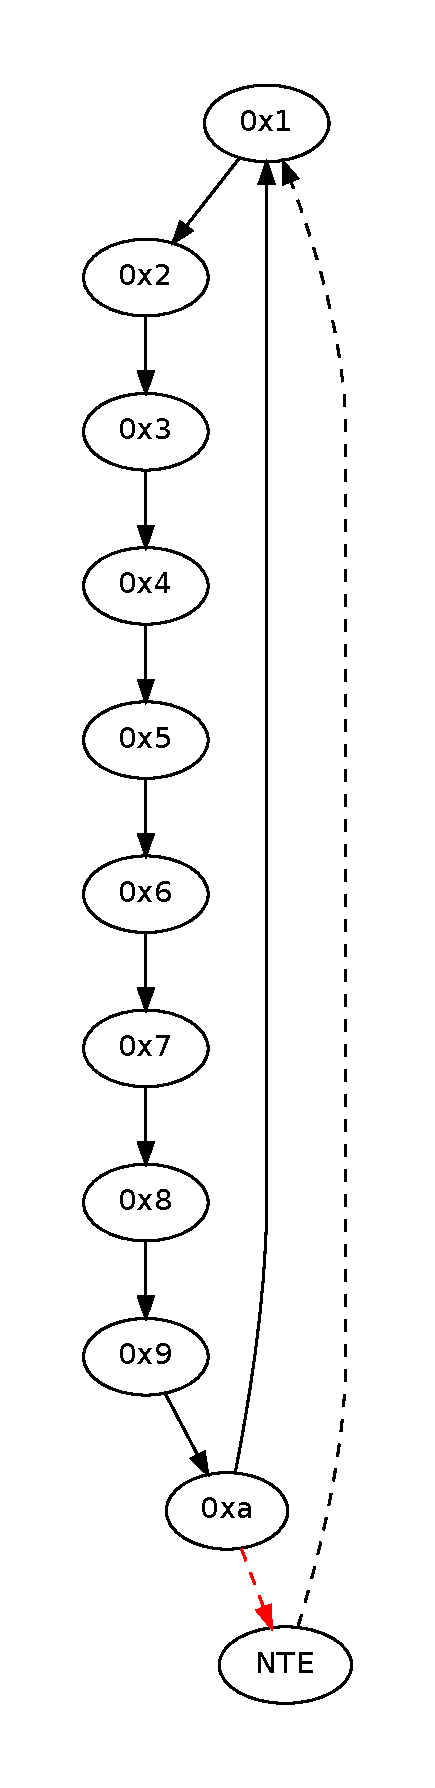
\includegraphics[scale=0.45]{./figs/validacao}
	\caption{}
	\label{fig-validacao}
\end{subfigure}

\caption{Código de validação e traço gerado.}
\label{valida_set}
\end{figure}


\section{Resultados}
Experimentos foram realizados com as técnicas de formação de regiões NET e MRET2, explorando as políticas de gerenciamento de \ccache~: \flush, \finefifo~e \coarsefifo~com granularidade 2, 4 e 8. 

Como para aplicações que cabem na \cache~a política de gerenciamento não faz diferença, e aqui estamos interessados em descobrir qual o comportamento do tradutor dinâmico de acordo a política de gerenciamento. Assim para todos os resultados neste artigo, é assegurado que o tamanho da \cache~é menor do que o necessário para armazenar todas as traduções da aplicação. Para isto, foram executadas simulações onde o tamanho máximo da \cache~é ilimitado, assim obtemos o Gráfico \ref{fig-cache-sizes}~, que mostra na primeira coluna o tamanho em \emph{bytes} necessários para armazenar todas as regiões de cada aplicação e na segunda coluna o número de instruções traduzidas.

\begin{figure}[!ht]
\centering
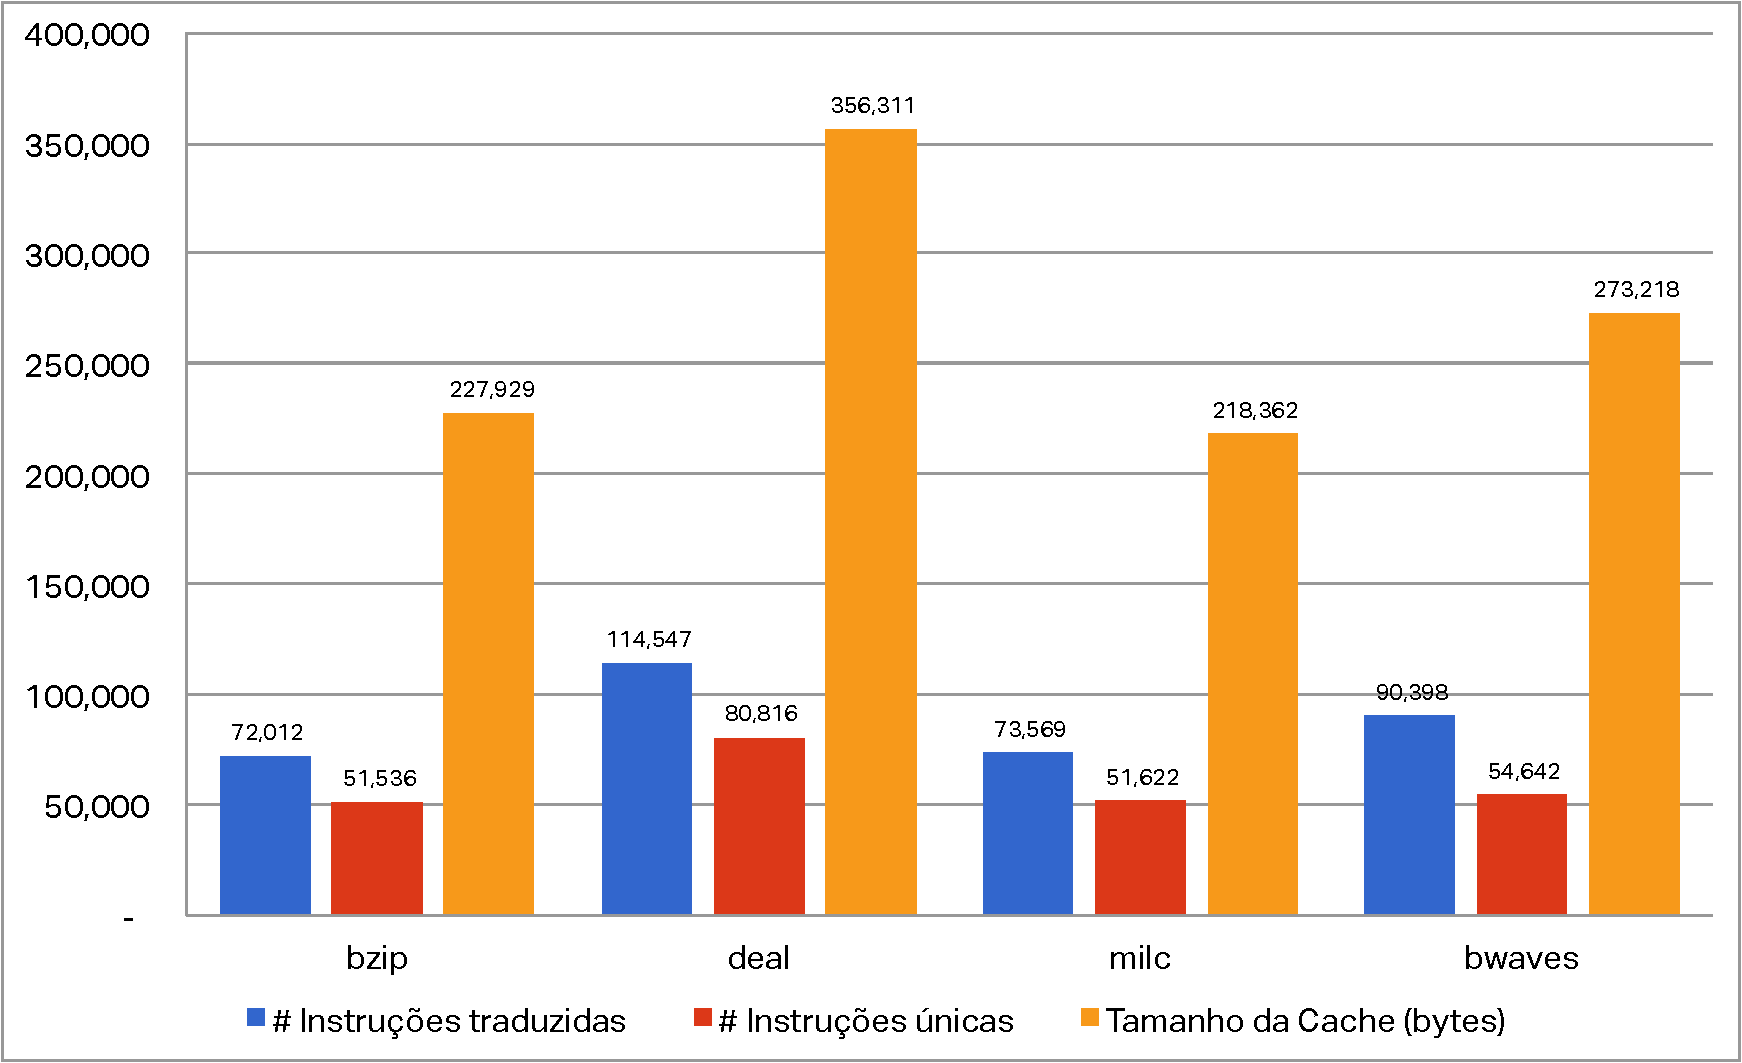
\includegraphics[scale=0.5]{./figs/cache-sizes}
\caption{Tamanho da cache sem política de gerenciamento.}
\label{fig-cache-sizes}
\end{figure}

Para assegurar o aumento da pressão na \cache, os tamanhos da \cache~foram calculados na forma $MaxCache/n$, onde $MaxCache$ é o tamanho em \emph{bytes} obtido ao executar a aplicação no simulador com um tamanho de \cache~ilimitado e n é um fator de pressão utilizado para assegurar que a política de gerenciamento está realmente em uso.


\subsection{Encadeamento de traduções}
Infelizmente, o ato de traduzir uma região para o conjunto de instruções do \emph{host} é uma tarefa relativamente custosa. Por este motivo, para compensar o custo de tradução, é desejável maximizar o tempo de execução dentro das regiões traduzidas, recorrendo o mínimo possível ao gerenciador de emulação.

Uma técnica bastante usada em máquinas virtuais, que reduz o impacto gerado pelos saltos entre as regiões traduzidas, é o \emph{chaining} - conhecido também como encadeamento. Esta técnica é caracterizada por substituir as chamadas para o gerenciador de emulação por instruções de saltos para as regiões alvos. O princípio consiste em verificar se o endereço alvo do salto foi previamente traduzido, e em seguida, inserir um trecho de código
%binário
responsável por efetuar o salto de forma direta e com o menor custo possível. Desta forma, as regiões são encadeadas dentro da \cache, evitando o desvio do fluxo de execução para o gerenciador de emulação.

Apesar da vantagem em encadear as regiões traduzidas, o \emph{chaining} afeta diretamente o desempenho da política de gerenciamento de \cache. Isso pois sempre que existe a necessidade de se remover uma região, será necessário desfazer todos os encadeamentos previamente construídos, cuja região a ser removida faz parte. Por este motivo, este trabalho buscou realizar experimentos com diferentes \emph{benchmarks}, na tentativa de verificar a quantidade de \emph{chains} gerados pelas técnicas de formação de região, quando combinados com diferentes políticas de gerenciamento de \cache.

Na Figura \ref{fig-milc-chain}~, podemos verificar o número de \emph{chains} removidos quando a pressão da \cache~sobe. É interessante notar que a medida que o número de agrupamentos da \coarsefifo~é aumentado, o desempenho passa a se aproximar da \finefifo~- conforme explicado na seção \ref{sec-codecache} -, removendo uma quantidade substancial de \emph{chains}. Devido ao fato de que a \coarsefifo divide a \cache em grupos, é natural que o aumento da granularidade faça com que os algoritmos apresentem um desempenho similar.

\begin{figure}[!ht]
\centering
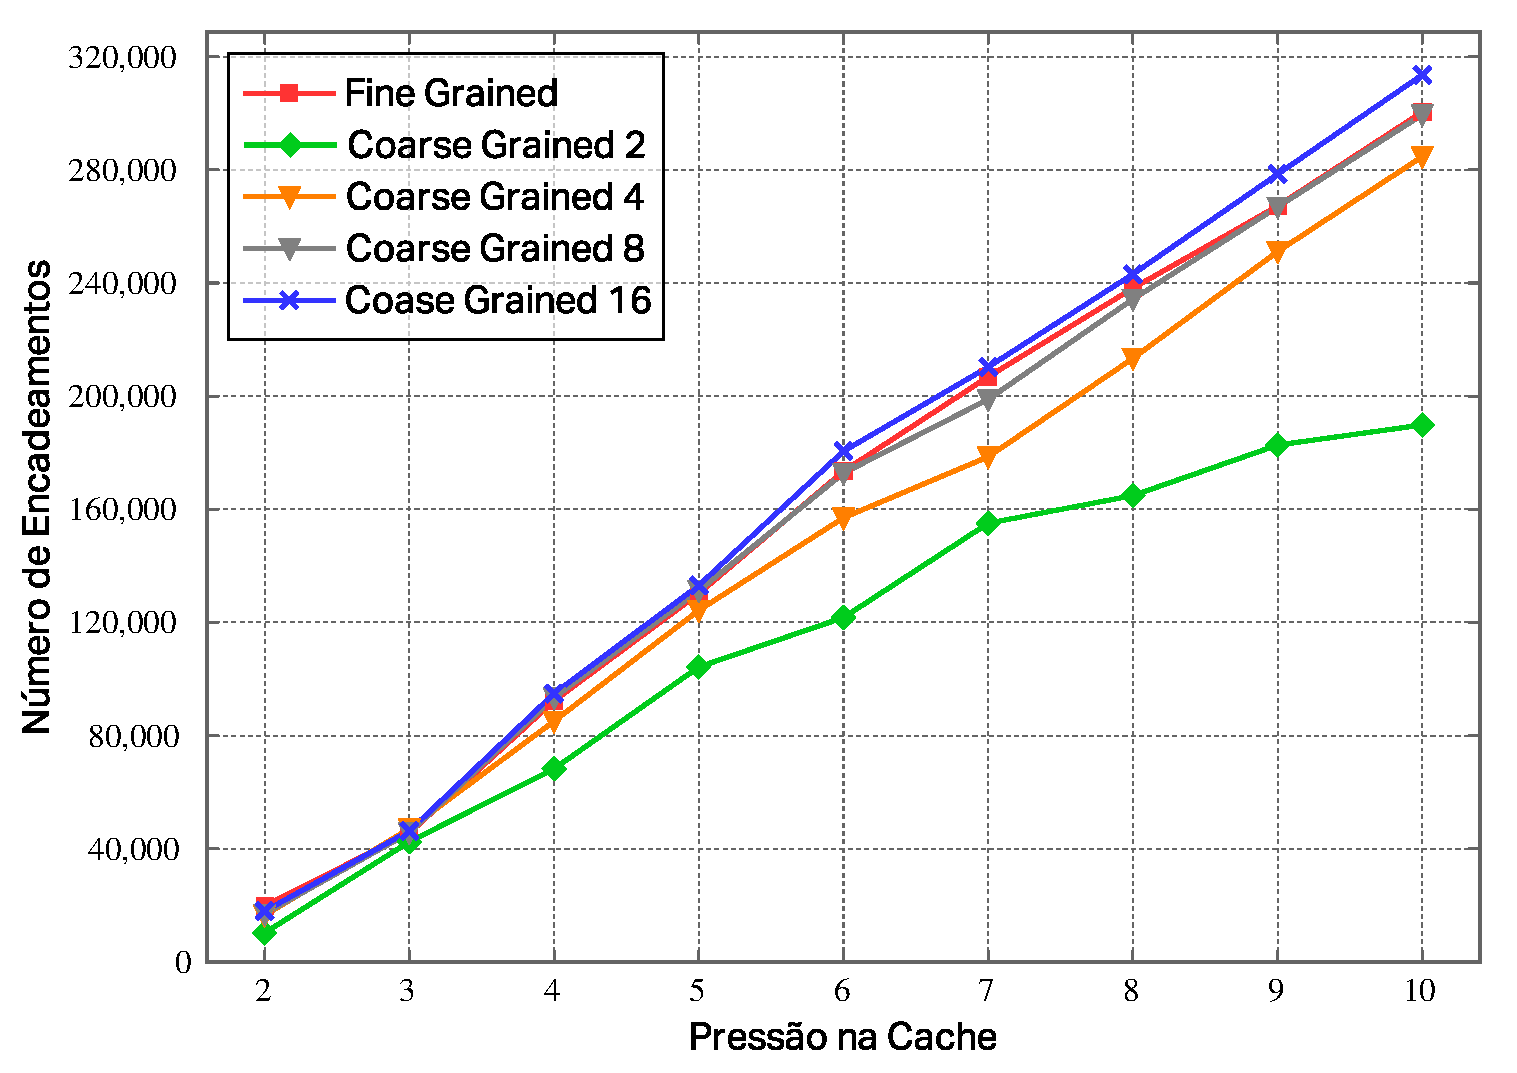
\includegraphics[scale=0.4]{./figs/net-milc-chaining}
\caption{Número de encadeamentos removidos para aplicação \emph{milc} e a técnica NET.}
\label{fig-milc-chain}
\end{figure}


Foi verificado ainda que, quando o número de agrupamentos chega a uma determinada proporção da \cache, seu desempenho começa a degradar, pelo fato da quantidade de elementos presente no tal agrupamento formar mais \emph{chains} entre as regiões fora dele do que que nas regiões internas a ele - pudemos verificar uma perda de desempenho bastante acentuada quando o agrupamento ultrapassou a granularidade $8$.


\subsection{Influência do \emph{profiler}}
Um dos grandes desafios na formação de regiões é a detecção de código quente, isto é, trechos em programas que são executados com grande frequência. O papel do \emph{profiler} é o de auxiliar o algoritmo de formação de regiões, armazenando estatísticas de execução de pontos específicos em um determinado programa. Esses pontos perfilados são escolhidos com base em uma condição previamente estabelecida, podendo por exemplo, ser imposta pelo algoritmo de formação de regiões. 

Como os programas de computador tendem a respeitar a localidade espacial e temporal, um perfilamento extremamente simples que pode ser aplicado é a contagem de vezes que um determinado endereço é executado. Contudo, é possível encontrar técnicas mais elaboradas, que fazem uso de propriedades estáticas dos binários, ou até mesmo, do comportamento das execuções anteriores de um dado programa.

Um dos problemas da abordagem de perfilamento adotada pelo RAIn é que todos os endereços, que são alvos de saltos, são perfilados sem respeitar as mudanças de fases dos programas. Isto é, a técnica de perfilamento usada pelo RAIn não prevê que em estágios de execução diferentes um mesmo endereço pode ser executado com um frequência menor que a apresentada em outras fases da aplicação. Essa característica, aliada a um perfilamento incremental, pode gerar regiões que não são realmente quentes em uma determinada fase da aplicação, aumentando o número total de regiões formadas e prejudicando a taxa de completude.

Além de apresentar um aquecimento incremental, a política de perfilamento original do RAIn não apresenta um resfriamento das instruções. Desta forma, após a remoção, a região removida continuará quente e quando for revisitada, será retraduzida.  Com isso, o número de regiões aumenta drasticamente, pois em determinadas fases do programa a região pode ser acessada com uma frequência muito menor que em fases anteriores, não sendo necessário uma retradução.

Buscando melhorar a abordagem de perfilamento adotada pelo RAIn, desenvolvemos duas técnicas de resfriamento do \emph{profiler}, o \emph{full reset} e o \emph{partial reset}. A técnica de \emph{full reset} consiste em resetar todos endereços perfilados sempre que uma região é criada. Isso garante que somente as regiões que são utilizadas muito frequentemente, em fases específicas do programa, consigam atingir o limiar mínimo necessário para serem consideradas quentes. Já as técnicas de \emph{partial reset}, reinicializa somente os contadores dos endereços que são alvos de salto e fazem parte das regiões. Isto garante que após a remoção de uma região, essa, por sua vez, só  poderá ser inserida novamente na \cache~quando atingir o limiar de aquecimento imposto pelo \emph{profiler}.

Com base nos experimentos realizados, verificamos que o total de traduções geradas pelo NET, na ausência de \cache~e fazendo uso da política original de perfilamento, é superior a taxa de traduções quando aplicamos algumas das técnicas de resfriamento sugeridas. Entretanto, na presença de \cache, a formação de regiões passa a ser afetada pela política de gerenciamento de \cache, sempre que há uma necessidade de liberar espaços para novas traduções. Assim, quanto maior a pressão sobre a \cache, mais regiões serão removidas, e consequentemente, mais instruções serão retraduzidas. Este efeito pode ser visualizado na Figura {\large Qual?}, onde a medida que a pressão sobre a \cache~cresce, o número total de instruções traduzidas aumenta. Contudo, este aumento é muito menor quando o perfilamento utiliza algumas das políticas de resfriamento sugeridas.

\begin{large}
NOVAMENTE FIGURA! O INTERESSANTE EH TER TODAS NO MESMO FORMATO!
\end{large}


É interessante notar, que apesar da redução do número total de traduções, a taxa de cobertura com o uso de um \emph{partial reset} é bem próxima da obtida pela política sem reset. Isso se deve ao fato, que o código gerado passa a apresentar uma taxa de completude muito superior, à medida que a pressão da \cache~aumenta, conforme visualizado na figura {\large Qual?}. Isso significa que com o resfriamento do \emph{profiler} as regiões são executadas completamente com uma maior frequência.



\subsection{NET e as políticas de gerenciamento de \emph{cache}}
\begin{large}
COLOCAR DEPOIS
\end{large}

\begin{large}
ABAIXO AS FIGURAS \ref{fig-num_regs}, \ref{fig-completude1} e \ref{fig-cobertura1} QUE COLOQUEI COMO MODELO, DEPOIS COMPLETAMOS AS OUTRAS
\end{large}

\begin{figure}[h!]
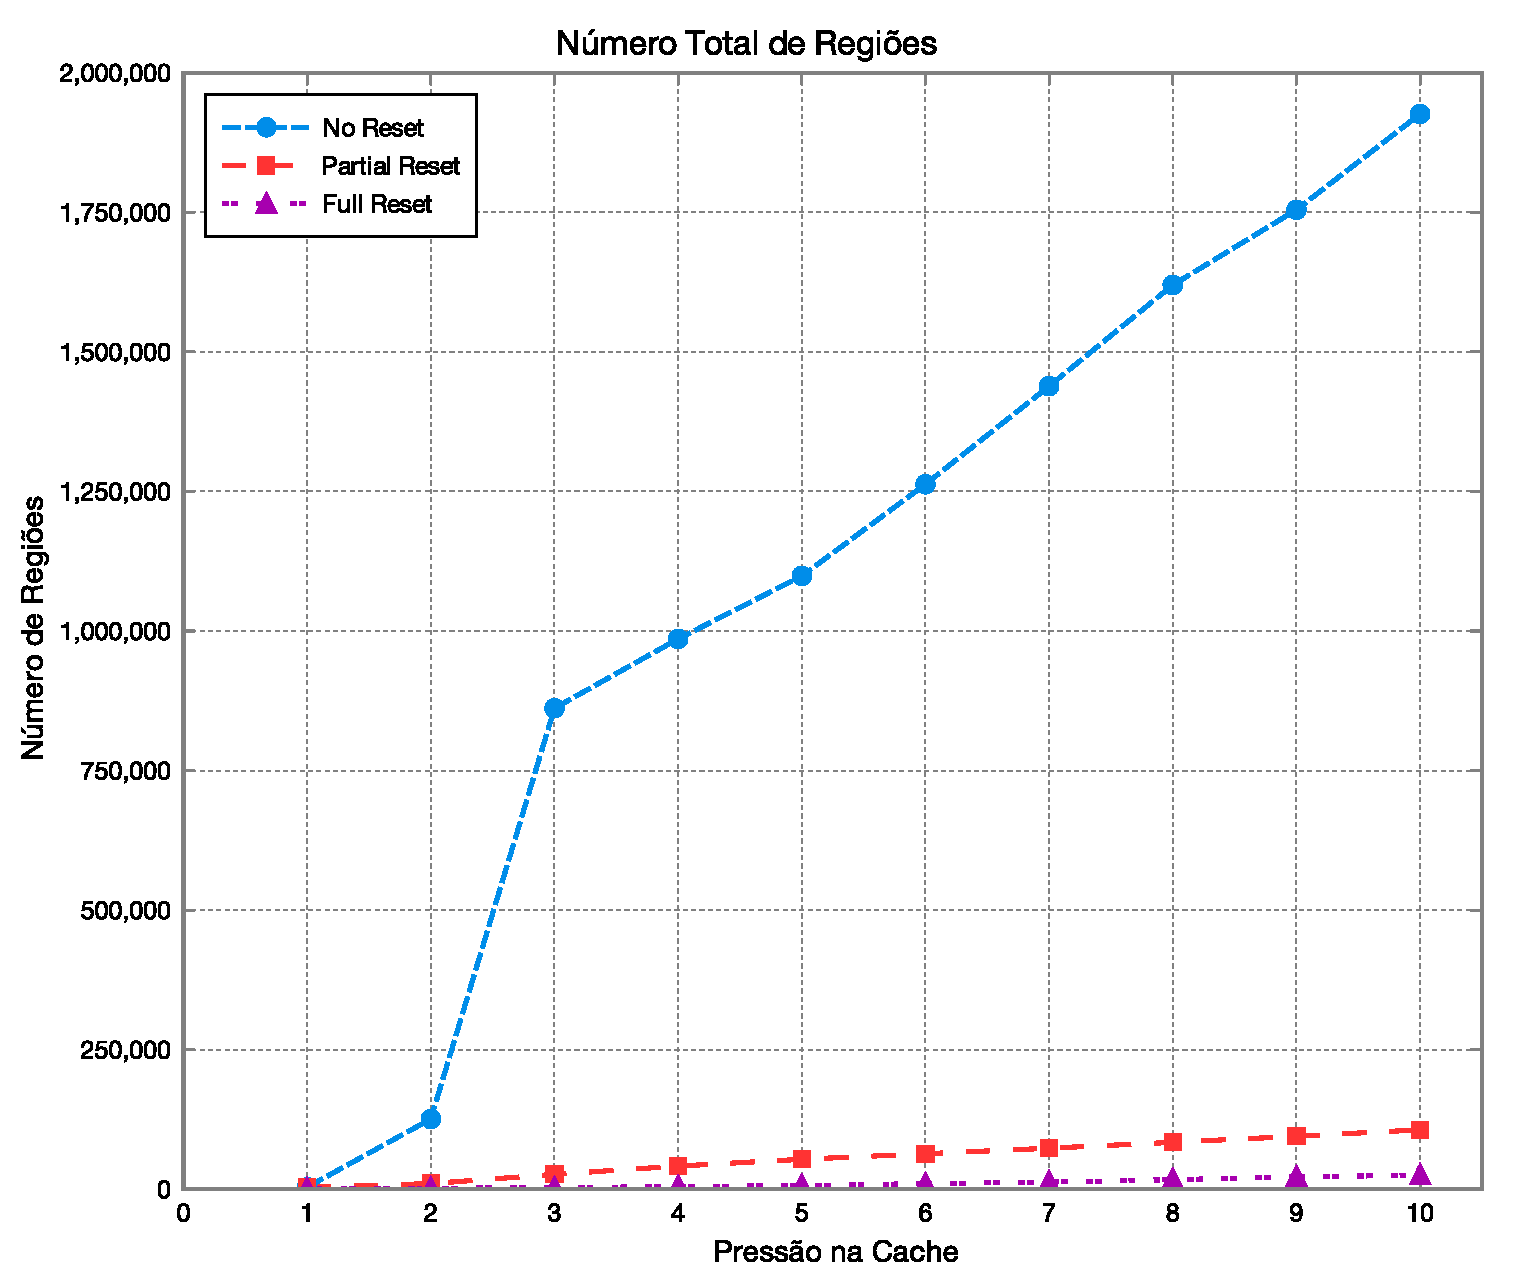
\includegraphics[scale=0.4]{./figs/regions-number}
\caption{Número de regiões.}
\label{fig-num_regs}
\end{figure}

Agora, 2 figuras lado a lado !

\begin{figure}[h!]
        \centering
        \begin{subfigure}[b]{0.45\textwidth}
                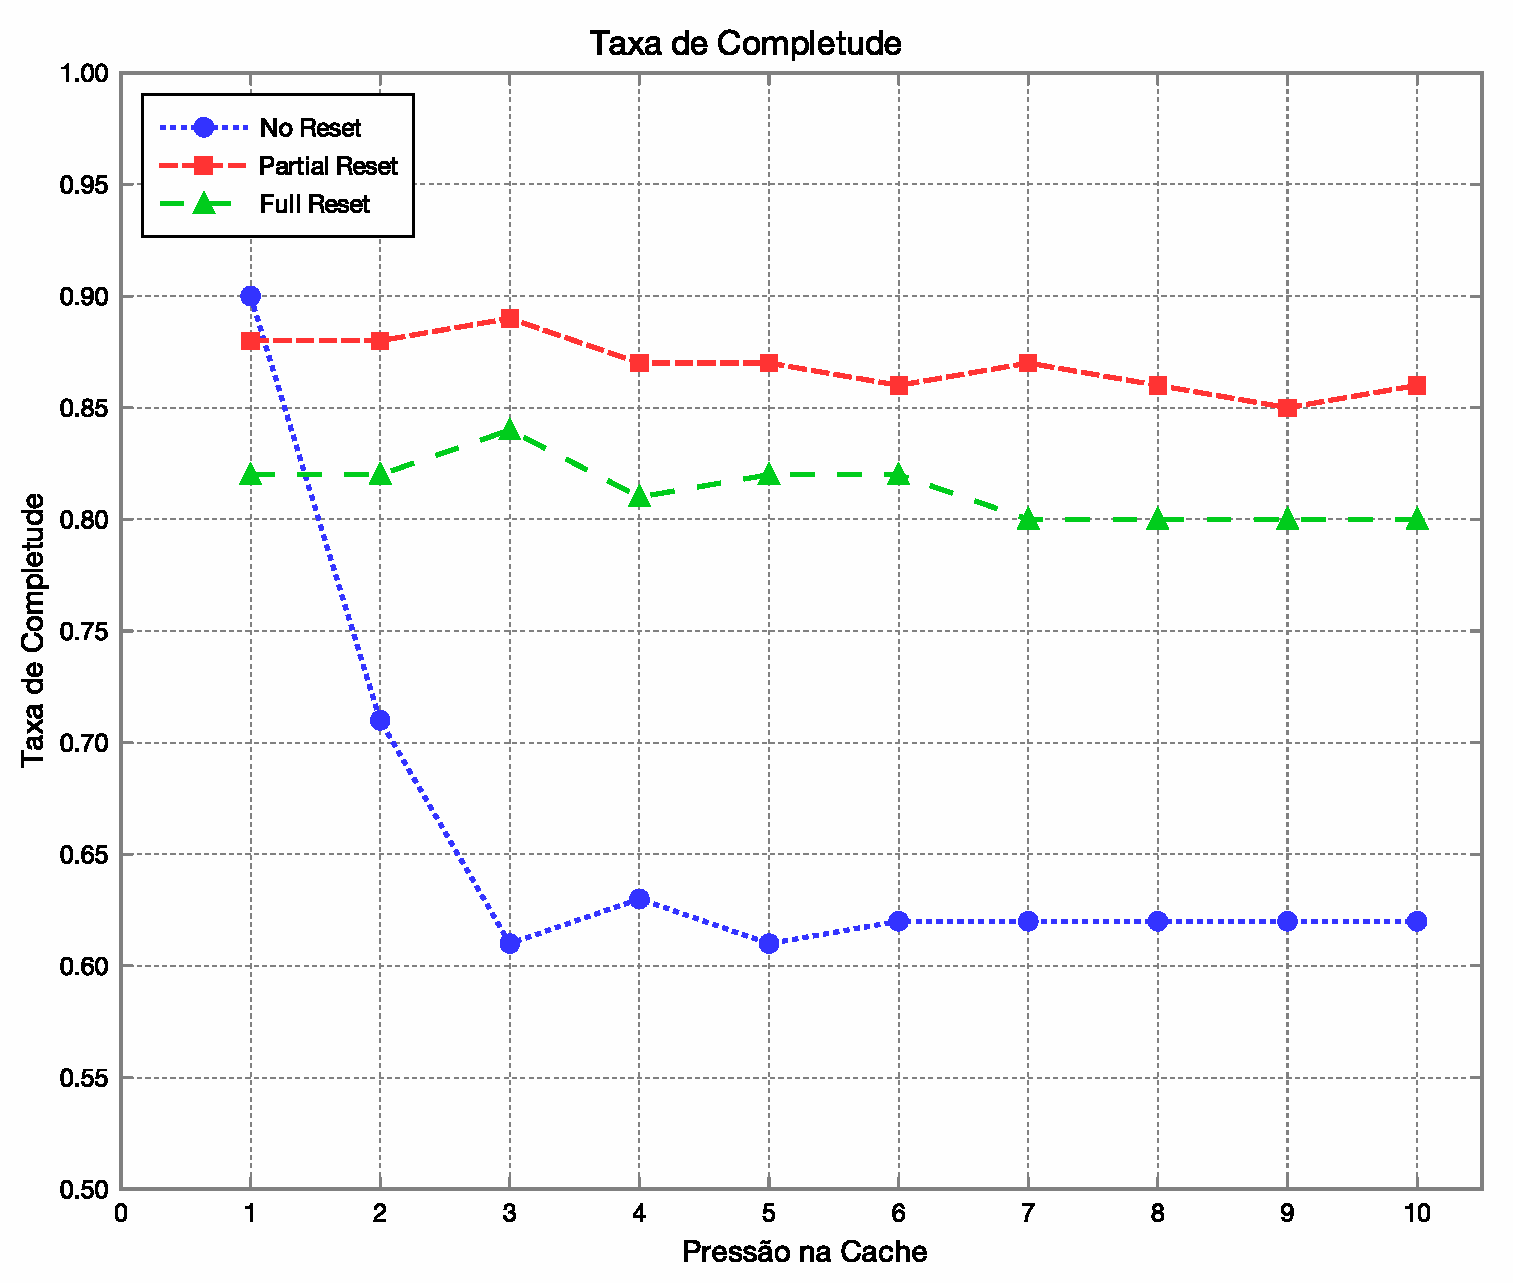
\includegraphics[width=\textwidth]{./figs/completion-reset}
                \caption{Completude}
                \label{fig-completude1}
        \end{subfigure}
        \quad %esapcço entre figuras - poderia ser \qquad ou nada...ou mais 100000 de coisas kkkkkkk
                \begin{subfigure}[b]{0.45\textwidth}
                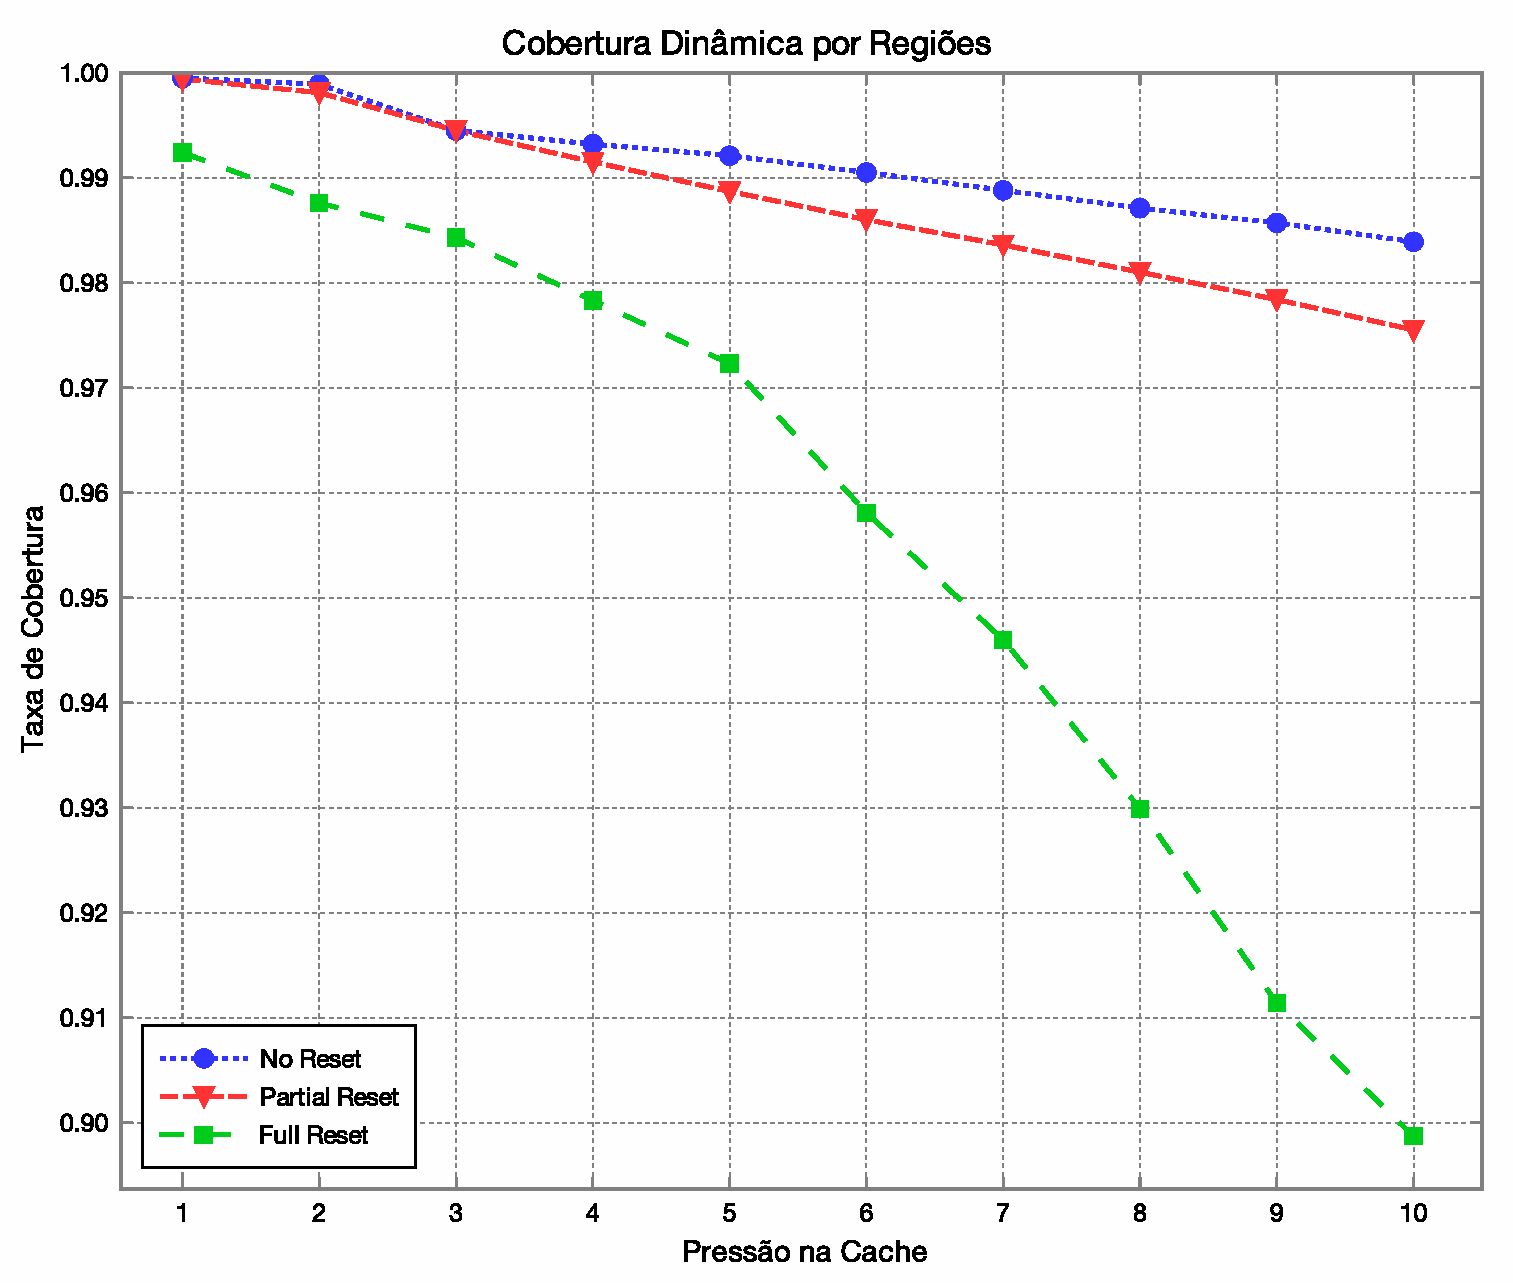
\includegraphics[width=\textwidth]{./figs/region-coverage-reset}
                \caption{Cobertura}
                \label{fig-cobertura1}
        \end{subfigure}
\caption{Dois graficos lado-a-lado...}
\end{figure}

\newpage

\section{Conclusões}
\begin{large}
A FAZER - DEPOIS Q A PARTE 5 ESTIVER PRONTA
\end{large}


% bibliografia
\bibliographystyle{ieeetr}
\bibliography{bibliografia}


\end{document}
